% XXX Jedes Jahr Professoren-Texte aktualisieren!
\section[Eure Profs stellen sich vor]{Eure Professoren stellen sich vor}
\textbf{Auf den folgenden zwei Seiten stellen sich eure beiden Professoren vor.
    Sie werden gemeinsam die "Physik~1" bis "Physik~3" lesen.
    Prof.\ Rohlfing wird sich dabei um die theoretischen und Prof.\ Wurstbauer um die experimentellen Aspekte des Studiums kümmern.
    Zudem stellt sich Prof.\ Werner vor, der die Vorlesungen "Mathematik für Studierende der Physik" halten wird (ebenfalls über drei Semester) und Dr. Kovarik, der sich in den ersten beiden Semestern um die Übungen kümmern wird.
	Da diese drei Professoren euch eine Zeit lang begleiten werden, ist es durchaus interessant zu wissen, was sie gemacht haben, bevor sie an die Uni Münster kamen, und wie ihre aktuelle Forschung aussieht.}

\begin{multicols}{2}
\begin{center}
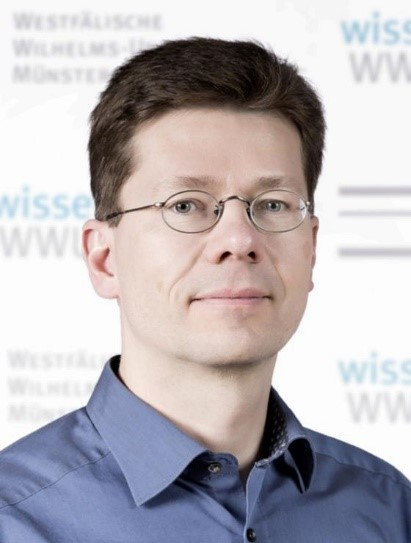
\includegraphics[width=0.71\columnwidth]{res/vorstellungsfotos/rohlfing.jpg}\\
Prof.\ Dr.\ Michael Rohlfing\\
Institut für Festkörpertheorie
\end{center}

Herzlich willkommen an der Universität Münster, am Fachbereich Physik und in unserem integrierten Kurs Physik 1-3! Meine Kollegin Ursula Wurstbauer und ich werden Ihnen gemeinsam die Grundlagen der Physik vermitteln - in experimenteller und theoretischer Hinsicht gleichermaßen.

Es mag Sie interessieren, dass ich selber vor 34 Jahren mein erstes Semester in genau denselben Räumen hier in Münster erlebt habe. Nach meinem Diplom und der Promotion verbrachte ich einige Zeit an der University of California in Berkeley und kam dann nach Münster zurück, um hier zu habilitieren. Dann verschlug es mich 2003 als frisch berufener Professor weiter nach Norden, erst nach Bremen und dann nach Osnabrück. 2013 kehrte ich wiederum nach Münster zurück, auf meine jetzige Stelle am Institut für Festkörpertheorie. Ich kenne also den Fachbereich aus sämtlichen Perspektiven.

In der Forschung befassen sich meine Arbeitsgruppe und ich mit Festkörperphysik, insbesondere mit Elektronenstrukturtheorie. Wir wenden unsere Methoden auf alles an, was man als "kondensierte Materie" bezeichnet: Moleküle, Polymere, Adsorbate auf Oberflächen, nanoskalig strukturierte Systeme, und seit einigen Jahren verstärkt zweidimensionale Materialien wie Graphen oder atomar dünne Halbleiter, etwa Molybdänsulfid. Die Elektronen bilden die chemischen Bindungen zwischen den Atomen und kontrollieren dadurch den strukturellen Aufbau der Materie. Vor allem aber interessieren uns die optischen Spektren, und dafür brauchen wir ebenfalls die Elektronen: wenn Sie einen Farbstoff sehen, sehen Sie letztlich deren quantenmechanische Zustände.

Diese Quantenmechanik werden Sie in Physik 1-3 nur in Ansätzen kennenlernen, denn unser Schwerpunkt liegt zunächst auf der klassischen Physik: Mechanik, Elektrodynamik, Thermodynamik. Aber auch in der mikroskopischen Welt werden Sie diese Dinge später wiederfinden: die Bewegung der Atome in einem Molekül ist in weiten Teilen durch klassische Mechanik geprägt, die Coulomb-Wechselwirkung zwischen Atomkernen und Elektronen gehorcht den Regeln der Elektrodynamik, und die thermodynamischen Eigenschaften auf der Mikroskala genügen denselben Grundkonzepten wie ein Ottomotor oder eine Wärmepumpe. Daher vermitteln wir Ihnen drei Semester lang diese immer noch gültigen Grundlagen, bevor es ab dem vierten Semester verstärkt in die "moderne" Physik gehen wird.

Ich wünsche Ihnen ganz herzlich einen guten Start in Ihr Studium, viele gute neue Freunde, tolle Erfahrungen und Eindrücke, viel Erfolg und ganz viel Spaß an der Physik!

\end{multicols}

\begin{center}
    \fibelimgtext{
	\includegraphics[width=0.7\textwidth]{res/xkcd/895_teaching_physics.png}
    }{\url{https://xkcd.com/895}}
\end{center}

\newpage

\begin{multicols}{2}
\begin{center}
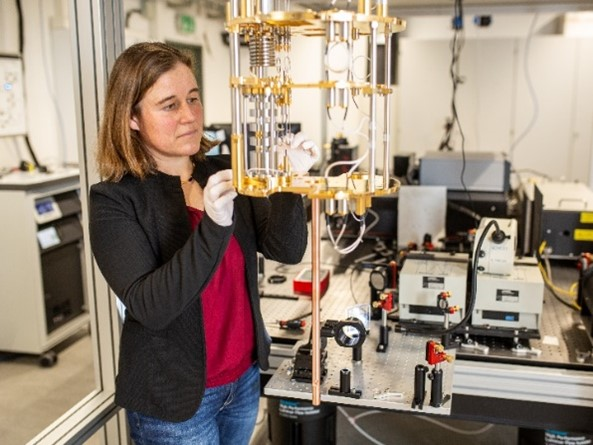
\includegraphics[width=0.8\columnwidth]{res/vorstellungsfotos/wurstbauer.jpg}\\
\smallskip
Prof.\ Dr.\ Ursula Wurstbauer\\
Physikalisches Institut
\end{center}

Auch von meiner Seite herzlich willkommen an der Universität Münster und insbesondere am Fachbereich Physik. Gleichzeitig möchte ich Ihnen zu Ihrer Entscheidung, das Physikstudium hier bei uns aufzunehmen, gratulieren. Sie dürfen im Laufe der kommenden Semester in die spannende, vielfältige Welt der Physik eintauchen.

Persönlich wollte ich zunächst Physik und Sport für das Lehramt an Gymnasien studieren, es war aber nur Physik und Mathematik möglich. So nahm ich zunächst dieses Studium an der Universität Regensburg auf. Schlüsselereignis, um neben dem Lehramts- auch den Physik-Diplomabschluss anzustreben, war ein Versuch im Fortgeschrittenenpraktikum zum Quanten-Hall-Effekt (Physik Nobelpreis 1986), bei dem wir selbst aus einem Stück Halbleiterkristall Mini-Drähte anlöteten, diese mit flüssigem Helium auf \SI{-269}{\celsius} abkühlten und bei großen Magnetfeldern das Experiment durchführten. So motiviert von der Arbeit im Labor und fasziniert von den Eigenschaften der Festkörper habe ich, nach erstem Staatsexamen und Physikdiplom, an der Uni Regensburg promoviert und bin dann nach einem ersten Postdoc an der Universität Hamburg für mehrere Jahre an der Columbia Universität in New York City tätig gewesen. Nach der Rückkehr aus den USA leitete ich an der TU München eine Nachwuchsgruppe und habilitierte. Seit 2019 bin ich nun an der WWU als Professorin am Physikalischen Institut tätig. 

Inhaltlich beschäftigen wir uns experimentell mit Anregungen in Quantum-/ Nanosystemen – derzeit meist in zweidimensionalen Kristallen. Dieses vielfältige Gebiet reicht von grundlegenden Eigenschaften in neuartigen Materialien, die beispielsweise zur solaren Energiegewinnung geeignet sind, über deterministisch erzeuge Quantenemitter, dem Verhalten neuartiger Supraleiter und anderen Quantenmaterialien. Dazu betreiben wir eine Reihe von Optik- und Transportlabore, nutzen Reinräume, um opto-/elektronische Schaltkreise und Proben herzustellen und haben im Labor mit < \SI{-272.12}{\celsius} (<\SI{10}{\milli \kelvin}) den kältesten Ort in Münster. 

Vielleicht waren sie zuletzt von Freunden oder der Familie mit der Frage konfrontiert: „Physik-Studium – und was macht man dann damit?“ Die Antwort ist meist nur im Zweifachbachelor-Studium (Lehramt) klar. Forschung, Entwicklung, Beratung, Versicherungen, Banken, Halbleiterindustrie, Automotive, Ingenieurwesen, Softwarearchitekt, ... Das ist nur eine unvollständige Berufsliste, in denen meine Alumni und Kommilitonen tätig sind. Denn was Sie auf jeden Fall lernen ist neben viel Physik und dem entsprechenden „Handwerkszeug“, komplexe Zusammenhänge zu erkennen und zu beschreiben, sich neue Themen zu erarbeiten, vielfältige Problemlösestrategien entwickeln, Arbeit im Team, teils im internationalen Umfeld - und eine hohe Frustrationstoleranz. Aber keine Sorge, der Spaß kommt dabei auch nicht zu kurz. Und so werden Sie zum begehrten Generalisten, dem nach dem Studium sehr viele Türen offenen stehen - natürlich und wichtig auch der Weg in das Lehramt.

Ich wünsche Ihnen viel Erfolg, gute Freunde und Kommilitonen und viel Spaß im Studium – und uns allen eine tolle gemeinsame Zeit in den Physik 1-3 Vorlesungen. 

\begin{center}
\includegraphics[width=0.85\columnwidth]{private/res/comics/manchmal_edited.jpg}\\
{\footnotesize 
S.~Harris – \url{sciencecartoonsplus.com}
}
\end{center}

\end{multicols}

\vfill

\newpage

\begin{multicols}{2}
\begin{center}
	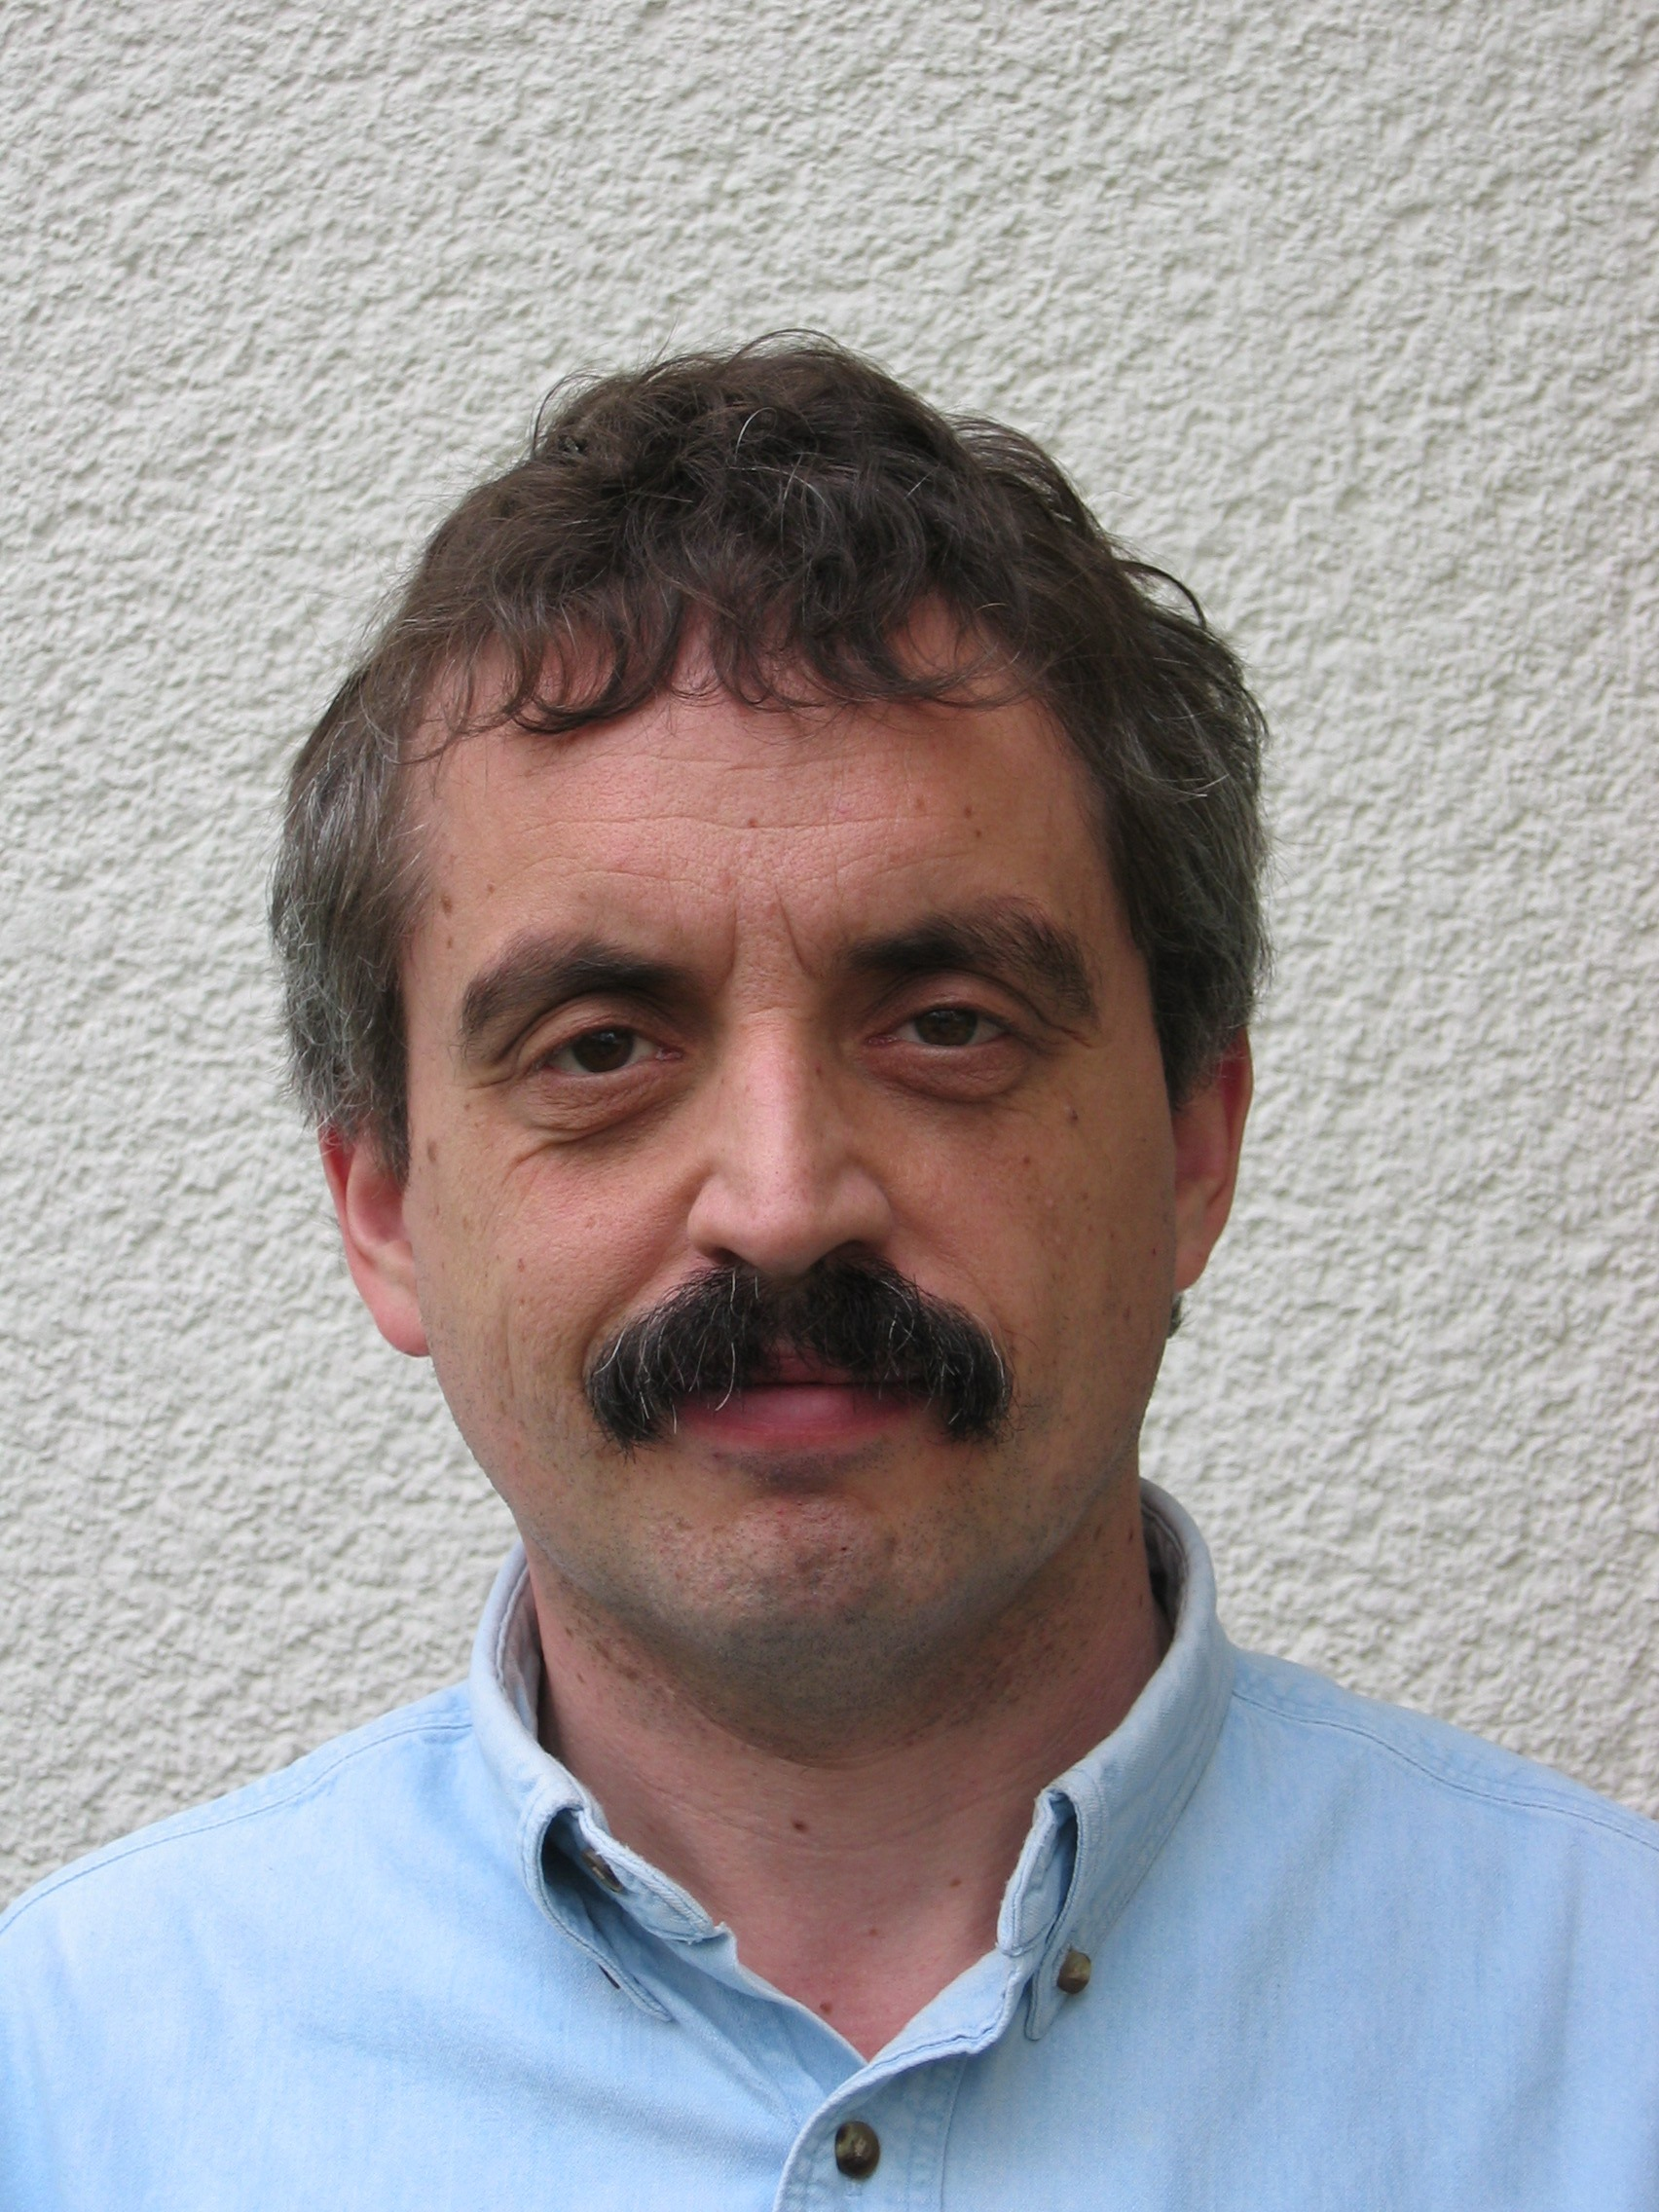
\includegraphics[width=\columnwidth, height=0.35\textheight]{res/vorstellungsfotos/wend_werner.jpg}\\
\smallskip
	Apl.\ Prof.\ Dr.\ Wend Werner\\
	Mathematisches Institut
\end{center}

Mir werden Sie in der nächsten Zeit in den Vorlesungen zur "Mathematik für Physiker" begegnen.
Mein Studium von Mathematik und Physik habe ich an der Freien Universität Berlin absolviert; Diplom und Promotion habe ich auch jeweils dort abgeschlossen.
Meine Habilitation habe ich an der Universität Paderborn gemacht und bin nun seit gut einem Jahrzehnt Hochschullehrer in Münster.

\[
	\resizebox{0.4\columnwidth}{!}{
		$\displaystyle\sum_{n = 1}^\infty \frac{1}{n^2} = \frac{\pi^2}{6}$
	}
\]

Die Themen von Promotion und Habilitation betrafen geometrische Fragen in Räumen unendlicher Dimension.
In letzter Zeit war das vor allem "Nichtkommutative Geometrie", ein Gebiet, welches versucht, einen mathematischen Formalismus zu finden, der in der Lage ist, Quanten- und relativistische Physik in einheitlicher Weise zu beschreiben.
Wie so oft beim Zusammenspiel von Mathematik und Physik sind auch hier interessante, rein mathematische Fragestellungen in Erscheinung getreten.

%\begin{center}
%	\includegraphics[width=\columnwidth, height=0.17\textheight]{private/res/comics/calvin_mathe.pdf}
%\end{center}

Der Zyklus "Mathematik für Physiker" ist eine kleine Herausforderung, da in vergleichsweise kurzer Zeit eine größere Stoffmenge vermittelt werden muss, die nichtsdestotrotz von den Teilnehmern anschließend handwerklich beherrscht werden muss.

Aber, keine Angst: Wir werden sehr langsam beginnen und erst im Laufe der Zeit Fahrt aufnehmen.
\end{multicols}

\begin{center}
	\fibelimgtext{
		\includegraphics[width=0.9\textwidth]{res/xkcd/435_purity.png}
	}{\url{https://xkcd.com/435}}
\end{center}
